\section{Continuous Symmetries}
\label{s:symm}

\subsection{Definitions}
\label{s:Definitions}

A dynamical system, $\dot{\ssp}=\vel(\ssp)$ is said to be \emph{equivariant} under the action of
an element $\LieEl$ of a continuous group if
\beq
	\vel( \ssp ) =  \LieEl^{-1}\vel( \LieEl \ssp )
	\,
\ee{equiv}

\noindent at every point in the \statesp\ \pS. Here we assume that $\LieEl$ is an element of a Lie group generated by the infinitesimal generator $\Lg$, 
such that $\LieEl(\theta) = e^{\theta \Lg}$, where $\theta$ parametrizes the group action. Condition \refeq{equiv} can equivalently be expressed as\rf{DasBuch}
\beq
  \groupTan(\vel(\ssp))  - \Mvar(\ssp) \, \groupTan(\ssp) =0
  \,,
\ee{inftmInv}

\noindent where $ \groupTan(\vel(\ssp)) = \Lg \vel(\ssp) $ is the group tangent of the velocity vector at \ssp, $ \groupTan(\ssp) = \Lg \ssp $ is the group tangent of $\ssp$ itself, 
and $\Mvar_{ij}(a)$ is the \stabmat\ ${\pde \vel_i}/{\pde\ssp_j} |_\ssp$.

% \ES{2014-05-15}{There is also a notational conflict between time $t$ and $\groupTan$, so that we have expressions like $\groupTan(\ssp)$ and $\ssp(t)$.
% Burak, please fix this by making a consistent choice.}
% \BB{}{I'm working on producing results, please have a look at \refref{BudCvi14}
% fix these following the conventions we used there.}


\label{s:relatives}

If the trajectory of a point $\ssp_\stagn$ coincides with its group
orbit, namely if one can find a group parameter $\theta (\zeit)$ such that
\beq
  \ssp_\stagn + \int_0^\zeit d\zeit' \vel(\ssp (\zeit')) = \LieEl (\theta (\zeit))\,\ssp_\stagn
  \,
\ee{releq}
for all $\zeit$, $\ssp_\stagn$ is called a \emph{\reqv}. By expanding both sides of \refeq{releq}
for infinitesimal time, we can get the relation
$\vel(\ssp_\stagn) = \dot{\theta}(\zeit) \Lg \ssp_\stagn$, which must hold for all $\zeit$. This means that $\dot{\theta}$ is a constant, which we call the \emph{\phaseVel} $c$. 
By multiplying through by $c$, the equivariance
condition \refeq{inftmInv} for \reqva\ can be compactly rewritten as
\beq
(\velRel \Lg - \Mvar ) \vel (\ssp_\stagn) = 0
\,.
\ee{ReqvMargEig}

We define a \statesp\ point $\ssp_\rpprime$ as lying on a \emph{\rpo} of period $\pd$ if its trajectory intersects its group orbit after time $\pd$, i.e.
\beq
  \ssp_\rpprime  + \int_0^\pd d\tau' \vel(\ssp (\tau')) = \LieEl (\theta_\rpprime ) \ssp_\rpprime
  \,,
\ee{relpo}
\noindent for some value $\theta_{\pd}$ of $\theta$. While the trajectory of a \rpo\ traces out the same path shifted
by the group action over and over again, as we will show in \refSect{s:numerics}, such a trajectory can be very complicated if the
continuous symmetry of the system is not reduced.

\subsection{\Mslices}
\label{s-slice}

In a system with $N$ continuous symmetries, a \emph{\slice} \pSRed\ is a codimension $N$ submanifold 
of \pS\ that cuts every group orbit once and only once. In the \emph{\mslices}, the solution
of a $d$-\dmn\ dynamical system is represented as a symmetry-reduced trajectory $\sspRed (t)$ within the
$(d-N)$-\dmn\ \slice\ and $N$ time dependent group parameters $\theta(t)$, which
map $\sspRed (t)$ to the full \statesp\ by the group action $\LieEl(\theta(t))$.

While this definition puts no restriction on the shape of the
\slice, it also provides no guidance on how to construct it.
In practice, a local approximation of the slice in the neighborhood of a point called a \emph{\slicePlane}
can be constructed by using the point $\slicep$ as \emph{\template\ }. The \slicePlane\ is then defined as the hyperplane
that contains $\slicep$ and is perpendicular to its group tangent $\sliceTan{} = \Lg \slicep$.
The relationships between \slicePlane s, \template s and reduced trajectories are illustrated schematically in \reffig{f-ReducTraj1}.
\DB{05.16.2014}{This is a comment for \reffig{f-ReducTraj1}. Formally, the two trajectories belong to the same \emph{wurst}, 
not the same group orbit. What terminology are we going to use going forward? Are we still happy with wurst or have we moved on?}
\ES{05.20.2014}{A wurst is a group orbit of a trajectory, so I do not think we need more terminology for this paper.
I also made the dependence of $\theta$ on $\tau$ explicit in the caption of \reffig{f-ReducTraj1} in order to stress the fact
that each point on the trajectory is rotated by different angle.}

%% ReducTraj*.* - read dasbuch/book/FigSrc/inkscape/00ReadMe.txt
\begin{figure}
\begin{center}
 \setlength{\unitlength}{0.40\textwidth}
 %% \unitlength = units used in the Picture Environment
 \begin{picture}(1,0.8361641)%
   \put(0,0){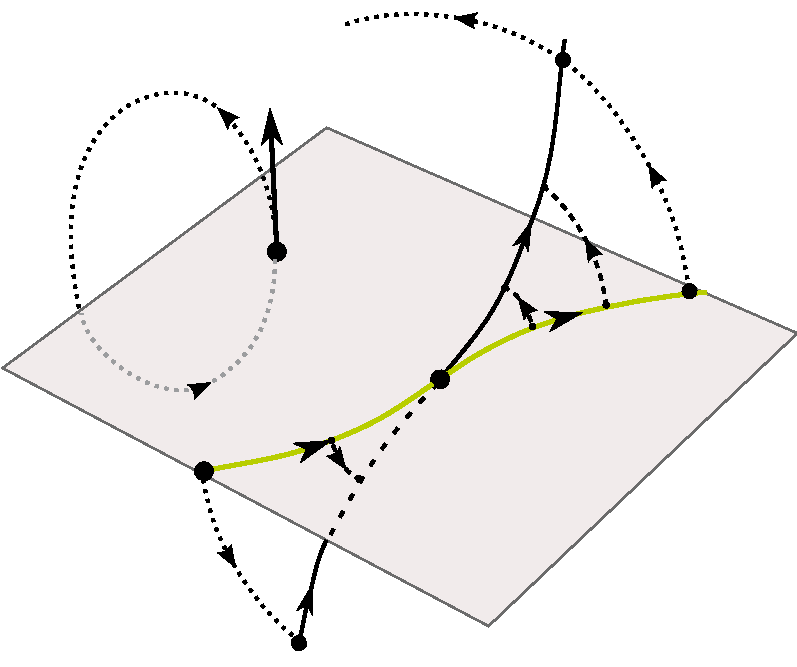
\includegraphics[width=\unitlength]{ReducTraj5.pdf}}%
   \put(0.06854399,0.36282057){\color[rgb]{0,0,0}\rotatebox{-30.34758661}{\makebox(0,0)[lb]{\smash{$\pSRed$}}}}%
   \put(0.57768586,0.29773425){\color[rgb]{0,0,0}\rotatebox{0.0313674}{\makebox(0,0)[lb]{\smash{$\sspRed(0)$}}}}%
   \put(0.59310014,0.69932675){\color[rgb]{0,0,0}\rotatebox{0.03136739}{\makebox(0,0)[lb]{\smash{$\ssp(\tau)$}}}}%
   \put(0.8268425,0.39772328){\color[rgb]{0,0,0}\rotatebox{0.03136739}{\makebox(0,0)[lb]{\smash{$\sspRed(\tau)$}}}}%
   \put(0.81220962,0.66529577){\color[rgb]{0,0,0}\rotatebox{0.03136739}{\makebox(0,0)[lb]{\smash{$\LieEl(\tau)$}}}}%
   \put(0.21150193,0.63610779){\color[rgb]{0,0,0}\rotatebox{0.0313674}{\makebox(0,0)[lb]{\smash{$\LieEl\,\slicep$}}}}%
   \put(0.37740434,0.49597258){\color[rgb]{0,0,0}\rotatebox{0.0313674}{\makebox(0,0)[lb]{\smash{$\slicep$}}}}%
   \put(0.3627714,0.69665188){\color[rgb]{0,0,0}\rotatebox{0.0313674}{\makebox(0,0)[lb]{\smash{$\sliceTan{}$}}}}%
 \end{picture}%
\end{center}
\caption{\label{f-ReducTraj1}The \slicePlane\ \pSRed\ is a hyperplane % \refeq{PCsect0}
passing through the {\template} point $\slicep$
and normal to its group tangent $\sliceTan{}$.
It intersects all group orbits (dotted lines) in an open
neighborhood of $\slicep$.  The full \statesp\ trajectory $\ssp(\tau)$ (solid black line) and the \reducedsp\
trajectory $\sspRed(\tau)$ (solid green line) belong to the same group orbit
$\pS_{\ssp(\tau)}$ and are equivalent up to a group rotation
$\LieEl\left(\ESedit{\theta(\tau)}\right)$ (from \wwwcb{}).
}%
\end{figure}

Reduced trajectories $\sspRed (t)$ can be obtained in two ways: by post-processing data
or by reformulating the dynamics and integrating directly on the \slice. In the post-processing method, which can be applied to both numerical and experimental data, 
one takes the data in the full \statesp\ and looks for the time dependent group parameter
that brings the trajectory $\ssp(t)$ onto the \slice. That is, one finds $\theta (t)$ such that $\sspRed(t) = \LieEl(- \theta (t)) \ssp (t)$ 
satisfies the \slice\ condition:
\beq
\braket{\sspRed(t) - \slicep}{\sliceTan{}} = 0
\,.
\ee{SliceCond}

In the second method, one reformulates the dynamics (for Abelian groups) as
\begin{subequations}\label{eq:so2reduced}
  \beq\label{eq:intSlice}
	\velRed(\sspRed) = \vel(\sspRed)
	-\dot{\theta}(\sspRed) \, \groupTan(\sspRed)
  \eeq
  \beq\label{eq:reconstruction}
	\dot{\theta}(\sspRed) = {\braket{\vel(\sspRed)}{\sliceTan{}}}/
				{\braket{\groupTan(\sspRed)}{\sliceTan{}}}
  \, ,
  \eeq
\end{subequations}
and computes $\sspRed (t)$ and $\theta (t)$ directly. In \refeq{eq:so2reduced}, $\velRed$ is the projection
of the full \statesp\ velocity \vel(\ssp) onto the \slicePlane. For a detailed derivation
of \refeq{eq:so2reduced}, see \refref{DasBuch}. Note that the time derivative
of the group parameter, which also appears in $\velRed$,
becomes singular if the dot product $\braket{\groupTan(\sspRed)}{\sliceTan{}}$
vanishes. We will refer the set of points on the \slicePlane\ which satisfy
\beq
\braket{\groupTan(\sspRed^*)}{\sliceTan{}} = 0
\,
\ee{ChartBordCond}
as the \emph{\sliceBord}.

%In general, \chartBord\ can be avoided by use of
%multiple \template s and arranging them in a way that the trajectories do not
%intersect the \chartBord , as done in \refref{atlas12}. In the particular
%case of the \twoMode\ system that we study in this paper, we can describe
%the reduced dynamics using a single \slice\ by picking a \template\ for which
%the \chartBord\ is a flow invariant subspace, hence never visited.

%If a $d$\dmn\ dynamical flow is $\Group$-equivariant under actions of
%an $N$ continuous parameters symmetry group $\Group$, its $d$\dmn\ \statesp\ is foliated
%by $N$\dmn\ group orbits, and the symmetry-\reducedsp\
%$\pS/\Group$ is $(d\!-\!N)$\dmn.
%The simplest continuous symmetry groups are the 1-parameter compact rotation
%group $\SOn{2}$ and the 1-parameter noncompact translation group
%$T(1)$; here we shall focus on the $\SOn{2}$ case.

So far, we have not put any constraints on the symmetry group that we are quotienting, 
beyond the requirement that it be Abelian\ES{2015-05-20}{Maybe you should discuss why
you imposed the restriction on Abelian groups.}.
From here on, we restrict our discussion to 1-parameter compact $\SOn{2}$
rotations that arise in spatially extended systems. \DBedit{In order to construct
a representation for $\SOn{2}$} \DB{}{What are we trying to say exactly here? Also does it make sense to make the function z and its coefficient $z_k$ so that the notation is consistent with the discussion about slice fixing in \refsect{s-slice2modes}} let us take a Fourier series expansion of
a real valued smooth periodic function:
\beq
	z(x,\zeit) = \sum\limits_{k=- \infty}^\infty z_k\left(\zeit\right) e^{i k x}, \,\,\,z_k = x_k + i y_k.
\ee{FourierSeries}
Truncating the expansion to $m$ modes, we
write the real and imaginary parts of the Fourier coefficients with
$k \geq 1$ as the state vector $\ssp = (x_1, y_1, x_2, y_2,..., x_m, y_m)$. The action of the $\SOn{2}$ group on this vector
can then be expressed as a block diagonal matrix:
%More explicit form, does not fit in a column:
%\beq
	 %\LieEl (\theta)= \\
					  %\begin{pmatrix}
					  %\cos \theta & \sin \theta & 0               & 0              & \cdots & 0              & 0               \\
					 %-\sin \theta & \cos \theta & 0               & 0              & \cdots & 0              & 0               \\
					  %0             & 0 		   & \cos 2 \theta & \sin 2 \theta & \cdots & 0              & 0               \\
					  %0             & 0            &-\sin 2 \theta & \cos 2 \theta & \cdots & 0              & 0               \\
					  %\vdots       & \vdots      & \vdots         & \vdots        & \ddots & \vdots         & \vdots         \\
					  %0             & 0 		   & 0               & 0              & \cdots & \cos m \theta & \sin m \theta  \\
					  %0             & 0            & 0	             & 0              & \cdots &-\sin m \theta & \cos m \theta
					  %\end{pmatrix}
%\eeq
\beq
	\LieEl(\theta) = \begin{pmatrix}
						R(\theta) & 0 			  & \cdots & 0 \\
						0		   & R(2 \theta) & \cdots & 0 \\
						\vdots	   & \vdots 	  & \ddots & \vdots \\
						0		   & 0	          & \cdots & R (m \theta)
					   \end{pmatrix} ,
\ee{mmodeLieEl}
where
\beq
	R(n \theta) =	\begin{pmatrix}
					\cos n \theta & - \sin n \theta \\
					\sin n \theta & \cos n \theta
					\end{pmatrix}
\ee{rotationmatrix}
is the rotation matrix for $n$th Fourier mode.
The Lie algebra generator for $\LieEl(\theta)$ is given by
\beq
	 \Lg =  \begin{pmatrix}
			 0 & -1 & 0 & 0 & \cdots & 0 & 0 \\
			 1 & 0 & 0 & 0 & \cdots & 0 & 0 \\
			 0 & 0 & 0 & -2 & \cdots & 0 & 0 \\
			 0 & 0 & 2 & 0 & \cdots & 0 & 0 \\
			 \vdots & \vdots & \vdots & \vdots & \ddots & \vdots & \vdots \\
			 0 & 0 & 0 & 0 & \cdots & 0 & -m \\
			 0 & 0 & 0 & 0 & \cdots & m & 0
			 \end{pmatrix} .
\ee{mmodeLg}

In order to construct a \slicePlane\ for such a system, let us choose the following \slice\ \template:
\beq
	\slicep = (1, 0, ..., 0) .
\ee{firstmodetemp}
The \slice\ condition \refeq{SliceCond} then constraints points on the reduced trajectory to the hyperplane given by
\beq
	\sspRed = (\hat{x}_1, 0, \hat{x}_2, \hat{y}_2, ..., \hat{x}_m, \hat{y}_m) .
\ee{slicetemp}
In order to satisfy the requirement that group orbits cross the \slice\ once and only once, we also restrict the \slicePlane\ to the half-space where $\hat{x}_1 > 0$. 
Without this requirement group orbits would pierce the \slicePlane\ twice. 
In general, a \slicePlane\ can be constructed by following a similar procedure for any choice of \template, allowing the symmetry 
reduction of the dynamics in a neighborhood of the \template\ bounded by the \sliceBord\ \refeq{ChartBordCond}. 
However, the power of choosing template \refeq{firstmodetemp} becomes apparent by analyzing the border of its \slicePlane. 
The points on \refeq{slicetemp} only lie on the \sliceBord\ if $\hat{x}_1 = 0$. 
This means that as long the dynamics are such that the magnitude of the first mode never vanishes, 
\emph{every} group orbit is guaranteed to have a unique representative point on the \slicePlane.

\footnote{Note that, in general, any template of the form $\slicep = (\hat{x}'_1, \hat{y}'_1, 0,...,0)$ would work just as well since the first mode has the symmetry of a circle. We picked the \slice\ \template\
\refeq{firstmodetemp} for computational convenience.} 
%

The \template\ \refeq{firstmodetemp} for $\SOn{2}$ was introduced by Budanur \etal~\rf{BudCvi14}
and is different from those used in the previous implementations
of the \mslices,\rf{rowley_reconstruction_2000,BeTh04,SiCvi10,FrCv11,atlas12,ACHKW11} in the sense that it is solely geometrical and it does
not necessarily carry any information about the dynamics
\ES{2014-05-20}{It's always a good idea to read the papers that we cite,
even though nowadays it's not mandatory (it seems).
The \template\ \refeq{firstmodetemp} is used in Sect. 6.2 of SiCvi10,
where it is called ``irreducible subspace slice.'' Moreover, you should
have a look at Olver\rf{OlverInv} (and cite\rf{FelsOlver98,OlverInv} 
for the postprocessing approach). Their typical choice of a slice is equivalent
to using \template\ \refeq{firstmodetemp}. }. 
More insight can be
gained by writing the symmetry-reduced evolution equations \refeq{eq:so2reduced}
explicitly for the template \refeq{firstmodetemp}:
\begin{subequations}
\beq
\velRed ( \sspRed )  = \vel(\sspRed)
   - \frac{\dot{y}_1\left(\sspRed\right)}{\hat{x}_1} \, \groupTan(\sspRed)
\label{e-so2red1stmode}
\,.
\eeq
\ESedit{
  \beq\label{eq:reconstruction1stmode}
	\dot{\theta}(\sspRed) = \frac{\dot{y}_1[\sspRed]}{\hat{x}_1}
  \, ,
  \eeq
}
\end{subequations}
\ESedit{
Noting that the angle of a point $(x_1,y_1)$ in the first Fourier mode plane is $\phi_1=\tan^{-1}\frac{y_1}{x_1}$, 
we find
\beq
  \dot{\phi}_1 = \frac{x_1}{r_1^2}\dot{y}_1-\frac{y_1}{r_1^2}\,\dot{x}_1\,,
\eeq
where $r_1=x_1^2+y_1^2$. Noting that on the slice, $\hat{y}_1=0$, we arrive at
\beq\label{eq:phi1}
  \dot{\theta}(\sspRed) = \dot{\phi}_1(\sspRed)\,.
\eeq
That is, for our choice of \template\ \refeq{firstmodetemp}, the reconstruction phase coincides with
the first Fourier mode phase. \ES{2014-05-20}{What would you think about introducing a functional
notation for $y_1$ as in \refeq{eq:reconstruction1stmode}?}
}


In general, one must be careful when the dynamics approach the \slice\ border $\hat{x}_1 = 0$. When this happens 
the near-divergence of $\velRed$ can be regularized by introducing a rescaled time coordinate such that
$d\hat{\zeit} = d\zeit / \hat{x}_1$\rf{BudCvi14}. However, in our study of the \twoMode\ system, we omit this
step since points with a vanishing first mode correspond to an invariant subspace of the flow and hence are never visited by the dynamics.

\subsection{Postproccessing approach}
\label{s-slice2modes}

\ES{2014-05-15}{This section refers to the ``method of moving frames'' (postprocessing approach)
and as such belongs here. It has to be generalized a bit (I will do it if you agree with the change).
Second mode \slice\ can be used also for integration on the \slice\ and can be introduced earlier.
}

\begin{figure}%[H]
\centering
 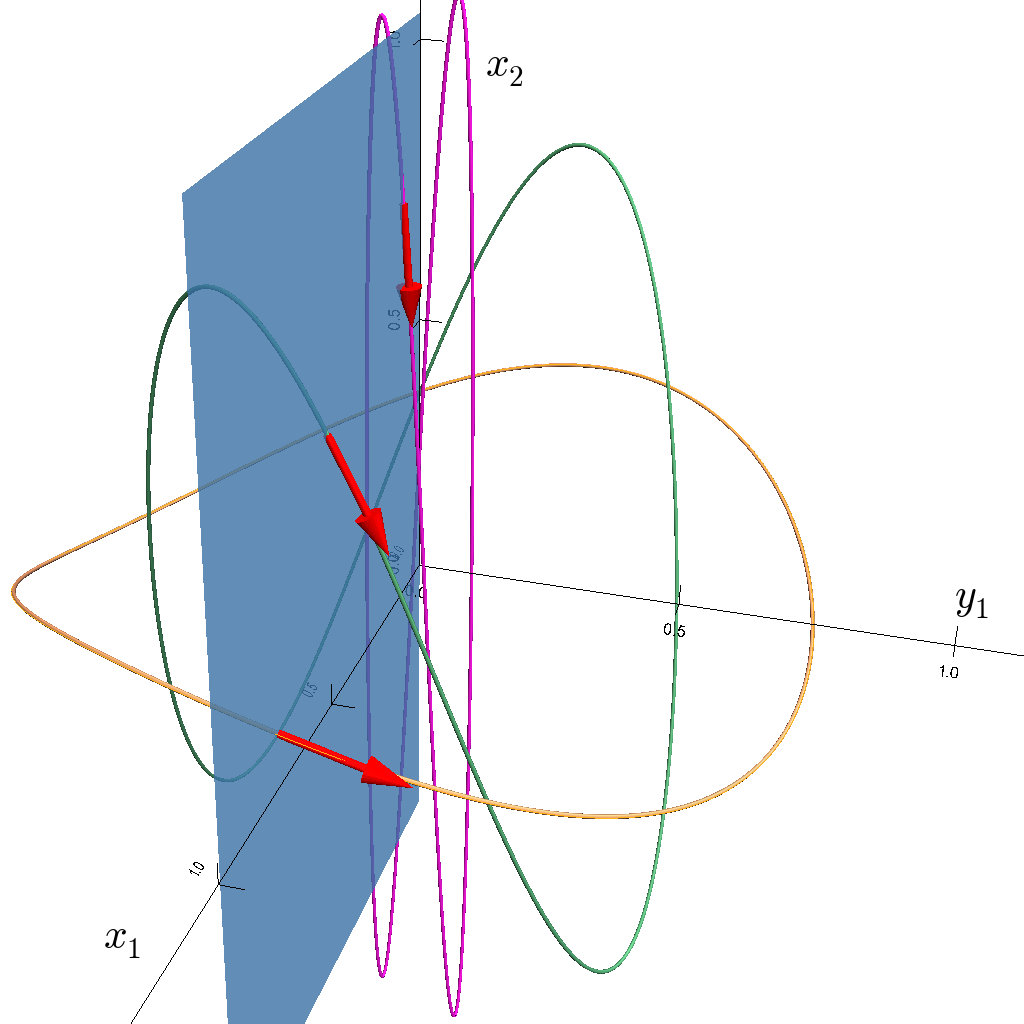
\includegraphics[width=0.45\textwidth]{BBgorbitsandslice}
\caption{$\SOn{2}$ Group orbits of \statesp\ points $(0.75, 0, 0.1, 0.1)$ (orange), $(0.5, 0, 0.5, 0.5)$ (green)
$(0.1, 0, 0.75, 0.75)$ (pink) and the first mode \slicePlane\
\refeq{slicetemp} (blue). The group tangents at the intersections with the \slicePlane\ are shown as red arrows.
As the magnitude of the first Fourier mode becomes small relative to the magnitude of the second one, the group tangent becomes more parallel to the \slicePlane.}
\label{fig:BBgorbitsandslice}
\end{figure}

In \refsect{s-slice}, we explained the general procedure for reducing
the \SOn{2} symmetry by \mslices. Here, we focus on its
geometrical interpretation using the \twoMode\
system as an example. The \slice\ defined by \refeq{firstmodetemp} and the directional
constraint $\hat{x}_1 > 0$ 
%
\DB{}{Think this should be $\hat{x}_1$. Revert to $x_1$ if I'm wrong.} 
%
fix the phase of the first complex Fourier mode to $0$. \Statesp\ points are related to their representative points on the \slicePlane\ by the following $\Un{1}$ action:
\beq
	\sspRedC_n = e^{-\ii n \phi_1} \sspC_n \, .
\ee{e-1stmodeTransform}
\DBedit{We immediately see that the reconstruction phase in \refeq{eq:so2reduced}
is, for this particular \slice, the phase of the first mode without the
symmetry reduction.} 
%
\DB{}{I don't immediately see what we are saying here. How does this relate to \refeq{eq:so2reduced}? I think this needs 
better explanation.}
\ES{}{It's not straightforward to see this, also for me, unless I think of the postprocessing
approach. So I have added \refeq{eq:phi1} above. Please check and discuss in
the blog if needed.}
%
The relation \refeq{e-1stmodeTransform} provides us
another interpretation for the \sliceBord :  For the template \refeq{firstmodetemp},
the \sliceBord\ condition \refeq{ChartBordCond} yields,
$|\sspRedC_1| = |\sspC_1| = 0$, which means that on the phase of the first Fourier
mode is not defined and \DBedit{the transformation \refeq{e-1stmodeTransform}
has no meaning.}
%
\DB{}{This phrase has no meaning.}
%
This is illustrated in \reffig{fig:BBgorbitsandslice}, which shows $3D$ projections of the
group orbits and group tangents of three reduced \statesp\ points. As the magnitude of the 
first mode, $\sqrt{\hat{x}_1^2 + \hat{y}_1^2}$, relative to that of the second mode becomes smaller, 
its group tangent has a larger component parallel to the \slicePlane. The \sliceBord\ condition
\refeq{ChartBordCond} is satisfied when the group tangent becomes parallel to the \slicePlane.
%
\DB{}{Don't love my wording of ``parallel to the \slicePlane'' since some people might interpret the 
\slicePlane\ as being defined by a vector normal to its surface and hence a perpendicular to the 
group tangent at the \sliceBord. However, I think that ``component that lies within the slice'' is
sort of vague and not well defined mathematically. What do you guys think?}


An immediate generalization of the transformation \refeq{e-1stmodeTransform},
is to fix the phase of a higher Fourier mode rather than that of the first one; this, however, requires
some extra care as we shall explain for the second Fourier mode.
Consider the phase-fixing transformation,
\beq
	\sspRedC_n = e^{-\ii n \frac{\phi_2}{2}} \sspC_n \, ,
	\label{e-2ndmodeTransform}
\eeq
which fixes the phase of the second mode to $0$. Note, however, that since
$\phi_2 \in (0, 2 \pi]$ it can have discontinuities of $2 \pi$. This means  
that when the first Fourier mode is transformed, it will have a phase discontinuity 
of $\pi$. This discontinuity can be fixed by another
transformation:
\bea
	\tilde{\sspC}_1 &=& e^{-\ii 2 \hat{\phi}_1} |\sspRedC_1 | \, , \continue
	\tilde{\sspC}_{n \neq 1} &=& \sspRedC_n \, ,
	\label{e-PhaseDoubling}
\eea
where we simply doubled the phase $\hat{\phi}_1$ of the symmetry-reduced
first mode $\sspRedC_1$, obtained by \refeq{e-2ndmodeTransform} and left
the rest of the modes unchanged. Combination of \refeq{e-2ndmodeTransform}
and \refeq{e-PhaseDoubling} is a valid symmetry reduction scheme since every
group orbit is represented by a single point, furthermore, it is also continuous
and revertible hence one can make further computations, such as constructing
Poincar\'{e} sections, using this form. For the 2-mode case at hand, representation
\refeq{e-PhaseDoubling} does not have any particular advantage against
\refeq{e-1stmodeTransform}, however, for higher dimensional flows, second
(or higher) Fourier mode subspaces can have dynamical importance as shown in
\refref{SCD07}. In order to capture those regions of the \statesp\ this
representation would be a useful alternative.

\subsection{Polar coordinates}
\label{s-polar}

In \refref{PoKno05}, a polar coordinate representation of \refeq{eq:DangSO2}
is obtained by defining the $\LieEl$-invariant phase: $\Phi = \phi_2 - 2 \phi_1$
and three symmetry invariant coordinates $(r_1, r_2 \cos \Phi, r_2 \sin \Phi)$.
One can see by direct comparison with \refeq{e-1stmodeTransform}, which
yields $\sspRedC_1 = r_1$ and $\sspRedC_2 = r_2 e^{\ii \Phi}$, that this
representation is a special case $(m=2)$, of the \slice\ defined by
\refeq{firstmodetemp}. Corresponding ODEs for the polar representation
were obtained in \refref{PoKno05} by  chain rule and substitution. Note
that \mslices\ provides a general form \refeq{e-so2red1stmode} for symmetry
reduced time evolution.
